The median OS in the entire population treated with CDK4/6 inhibitors was 46 months (95\%CI 39.4–55.6). Median PFS was 20.1 months (95\%CI 18.3–24.2). Following this, we compared Palbociclib and ribociclib only as first-line treatments. We found that regarding OS, there is no significant difference between the two, but ribociclib is significantly better in terms of PFS (p-value $leq$ 0.001) (Figure \ref*{fig:interest}). Additionally, we compared the same CDK4/6 inhibitors with letrozole as a combination only (PAL-LT and RIB-LT). Regarding this scenario, we found out that both were similar in terms of OS and PFS.


\begin{figure}[ht]
  \caption{Survival curves for Palbociclib and Ribociclib (1st line) - Progression Free Survival and Overall Survival}\label{fig:interest} 
  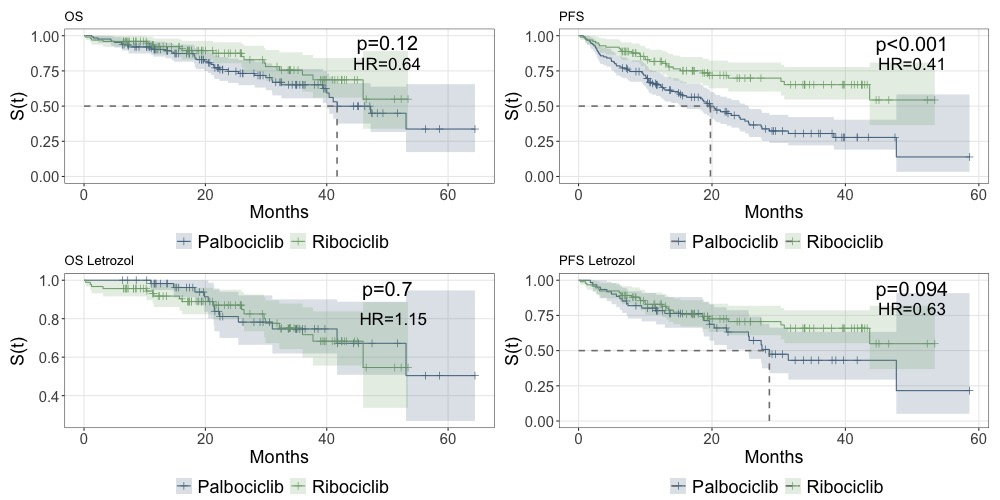
\includegraphics[scale=0.45]{figures/interest_curve_both.jpeg}%

\end{figure}


We then compared both with a cox regression, where OS shows no significant difference between palbociclib and ribociclib when adjusted to the stage, visceral metastases, age, treatment line, combination and ECOG. The proportional hazards' assumption was confirmed with p values all over 0.10.
\begin{table}[ht]
  \centering
  \caption{Cox Regression with palbociclib and Ribociclib - Progression Free Survival and Overall Survival}\label{tab:cox} 
  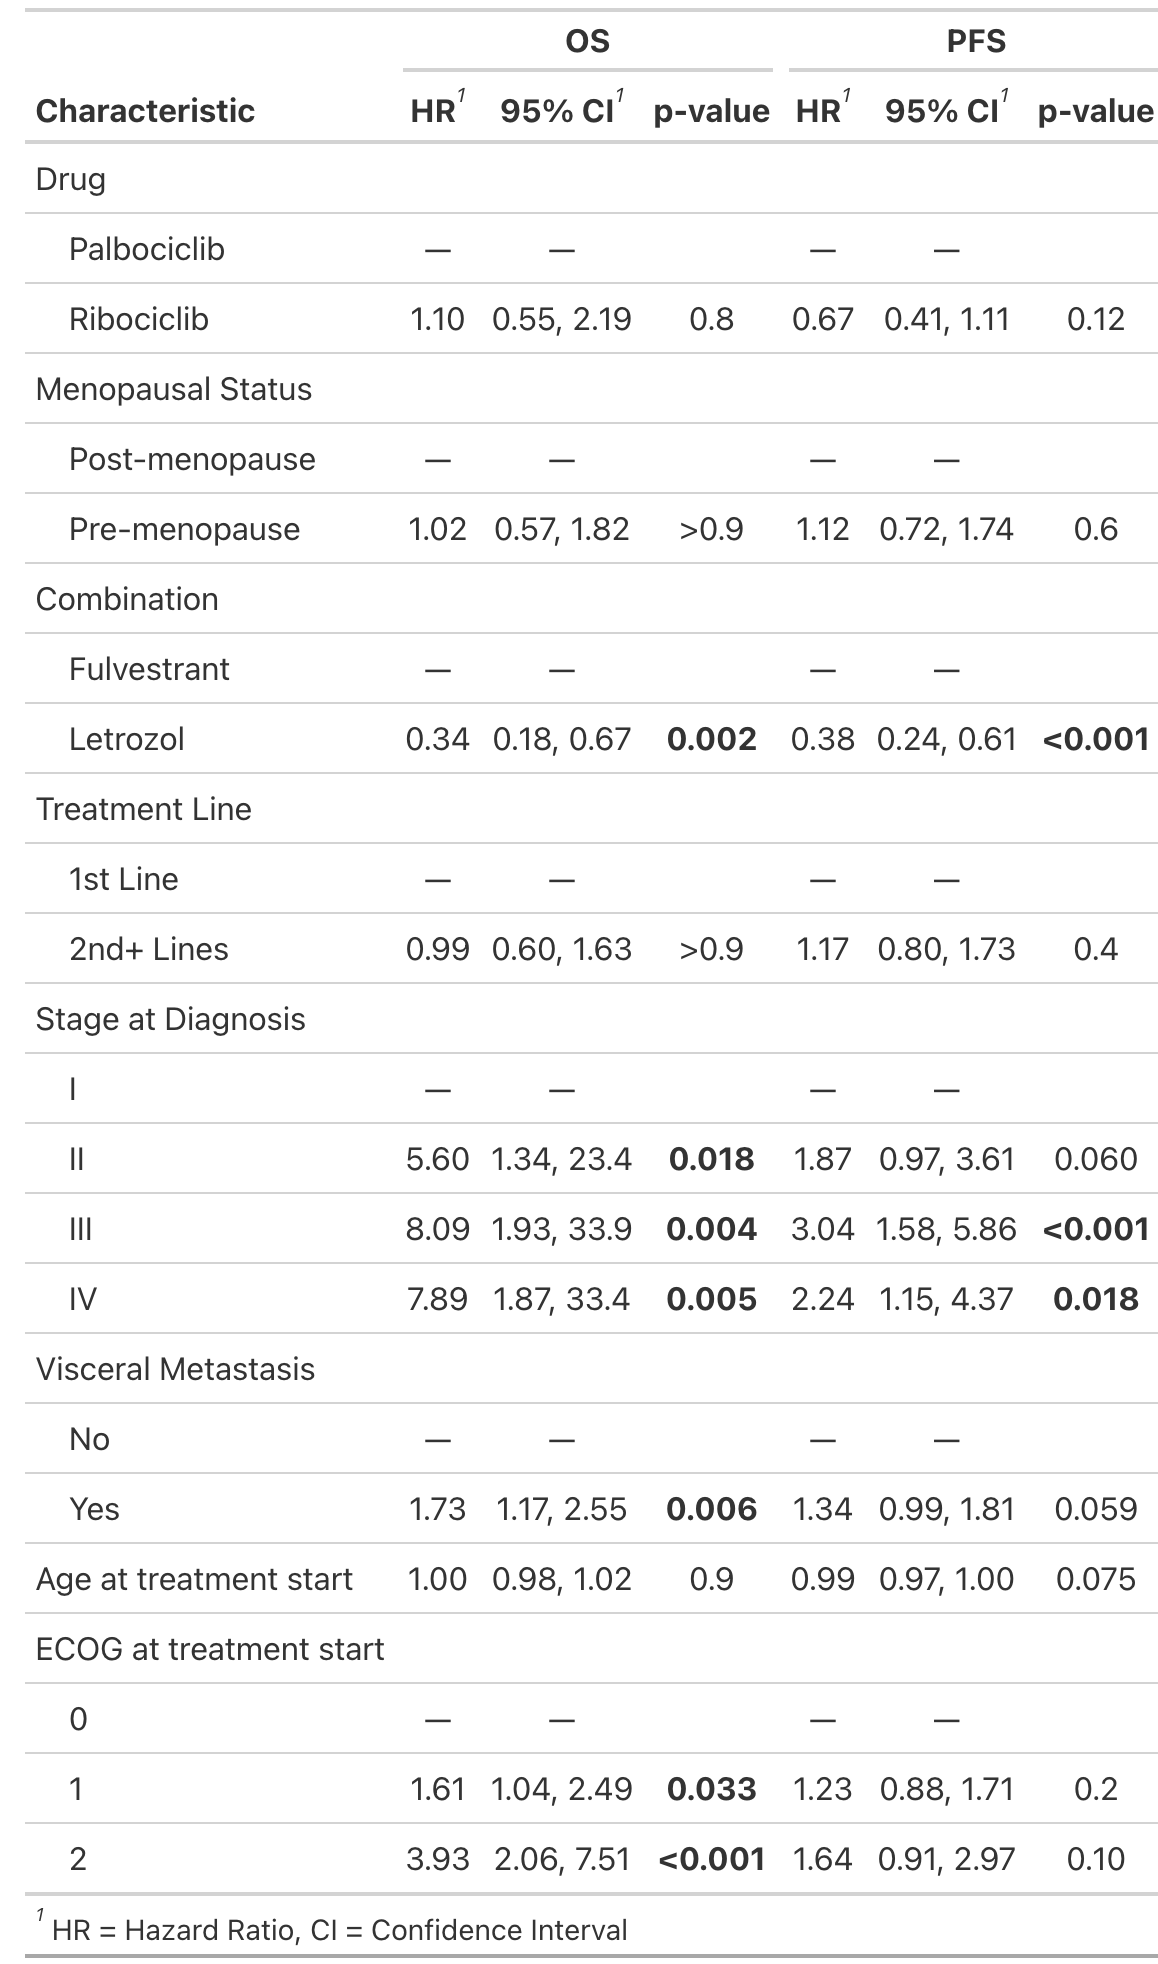
\includegraphics[scale=0.20]{figures/cox_both.png}%

\end{table}

When comparing endocrine therapy with CDK4/6 inhibitors as first-line treatment (figure 2). For this study we only compared patients with bone only metastasis. When comparing both CDK4/6i combined with Fulvestrant or letrozole, we see that  Ribociclib (RIB+LT/FUL) is significantly better for PFS (p-value $leq$ 0.001 HR=0.21) but not OS. For Palbociclib as the first line with Fulvestrant or letrozole (PAL+LT/FUL), we see that there is no significant difference in terms of PFS and OS (p=0.57 and 0.51). We also applied the same analysis but comparing only the letrozole combination with letrozole alone (PAL-LT/RIB-LT vs LT). We found that both ribociclib and palbociclib are significantly better in terms of PFS (HR 0.65 for palbociclib and 0.27 for ribociclib) but not OS.
\begin{figure}[ht]
  \centering

  \caption{Survival curves (OS and PFS) comparing endocrine therapy (ET) to CDK4/6 inhibitors combined with fulvestrant or letrozole as 1st line. First row is CDK4/6i combined fulvestrant or letrozole vs fulvestrant or letrozole. Second row is CDK4/6i combined with letrozole vs letrozole alone. p values shown as pairwise vs. ET.  }\label{fig:grouped} 
  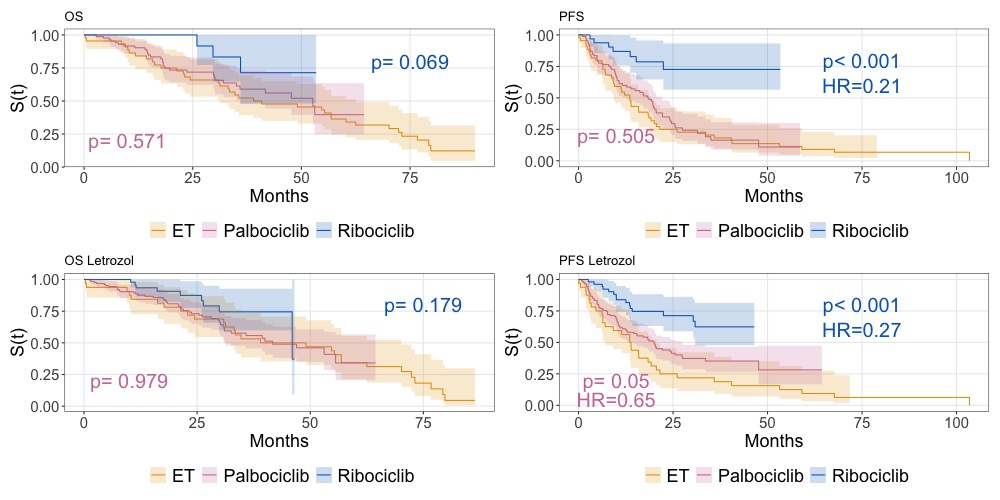
\includegraphics[scale=0.42]{figures/grouped_curve_both.jpeg}%

\end{figure}

When comparing palbociclib and ribociclib adjusted for ATE weights, we found a different scenario from previous assessments. There is a significant difference between the two in terms of OS (figure \ref*{fig:propensity}). The weights were calculated as stated in the methods section.


\begin{figure}[ht]
  \centering

  \caption{Comparison of palbociclib and ribociclib survival curves adjusted for propensity scores  }\label{fig:propensity} 
  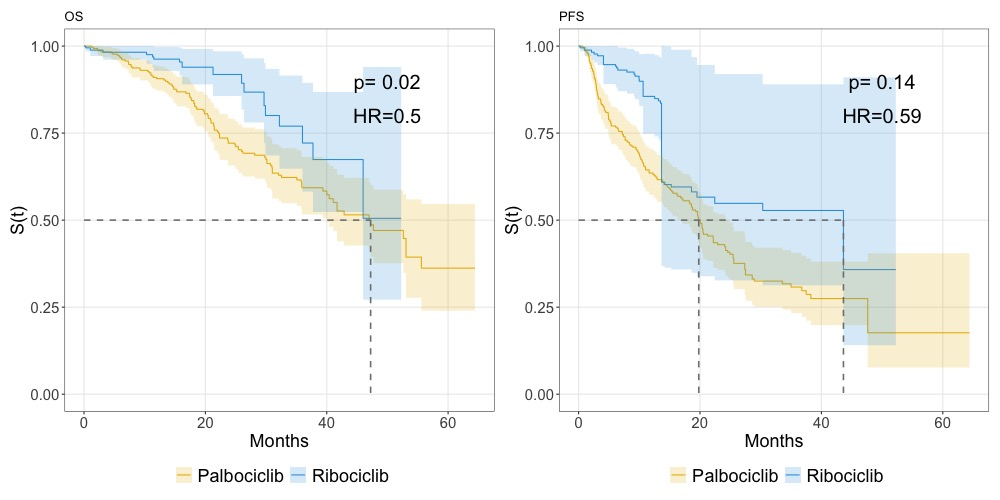
\includegraphics[scale=0.42]{figures/propensity_score_both.jpeg}%

\end{figure}

The Cox regression adjusted for the variables and with the weights applied to render an HR=0.55 [95\% CI 0.28-1.09;p=0.086] for OS. The HR for PFS is 0.56 [95\% CI 0.32-1;p=0.05].